\subsection{Identified}
\label{sec:Identified}

All SBOL-defined classes are directly or indirectly derived from the \sbol{Identified}  abstract class.
This inheritance means that all SBOL objects are uniquely identified using \sbol{URI}s that uniquely refer to these objects within an SBOL document or at locations on the World Wide Web.

As shown in \ref{uml:identified}, the \sbol{Identified} class includes the following properties: \sbol{displayId},  \sbol{name}, \sbol{description}, \sbol{prov:wasDerivedFrom}, and \sbol{prov:wasGeneratedBy}. 

\begin{figure}[ht]
\begin{center}
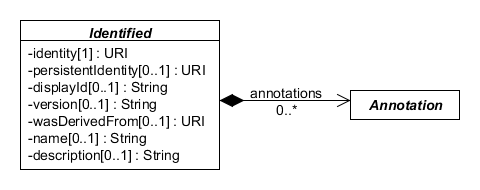
\includegraphics[scale=0.6]{uml/identified}
\caption[]{Diagram of the \sbol{Identified} abstract class and its associated properties}
\label{uml:identified}
\end{center}
\end{figure}
  
\subparagraph{The \sbolheading{displayId} property}
\label{sec:displayId}
The \sbol{displayId} property is an OPTIONAL identifier with a data type of \sbol{String}. This property is intended to be an intermediate between a URI and the \sbol{name} property that is machine-readable, but more human-readable than the full URI of an object.

If the \sbol{displayId} property is used, then its \sbol{String} value MUST be composed of only alphanumeric or underscore characters and MUST NOT begin with a digit.

\subparagraph{The \sbolheading{name} property}
\label{sec:name}

The \sbol{name} property is OPTIONAL and has a data type of \sbol{String}. This property is intended to be displayed to a human when visualizing an \sbol{Identified} object.

If an \sbol{Identified} object lacks a name, then software tools SHOULD instead display the object's \sbol{displayId} or URI.
It is RECOMMENDED that software tools give users the ability to switch perspectives between \sbol{name} properties that are human-readable and \sbol{displayId} properties that are less human-readable, but are more likely to be unique.

\subparagraph{The \sbolheading{description} property}
\label{sec:description}

The \sbol{description} property is OPTIONAL and has a data type of \sbol{String}. This property is intended to contain a more thorough text description of an \sbol{Identified} object.

\subparagraph{The \sbolheading{prov:wasDerivedFrom} property}
\label{sec:prov:wasDerivedFrom}
An \sbol{Identified} object can have zero or more \sbol{prov:wasDerivedFrom} properties, each of type URI. This property is defined by the PROV-O ontology and is located in the \url{https://www.w3.org/TR/prov-o/} namespace (Reference: \ref{sec:provenance}).

 An SBOL object with this property refers to one or more SBOL objects or non-SBOL resources from which this object was derived. An SBOL object MUST NOT refer to itself via its own \sbol{prov:wasDerivedFrom} property or form a cyclical chain of references via its \sbol{prov:wasDerivedFrom} property and those of other SBOL objects. For example, the reference chain ``$A$ was derived from $B$ and $B$ was derived from $A$'' is cyclical.

\subparagraph{The \sbolheading{prov:wasGeneratedBy} property}
\label{sec:prov:wasGeneratedBy}
An \sbol{Identified} object can have zero or more \sbol{prov:wasGeneratedBy} properties, each of type URI. This property is defined by the PROV-O ontology and is located in the \url{https://www.w3.org/TR/prov-o/} namespace (Reference: \ref{sec:provenance}).

An SBOL object with this property refers to one or more \sbol{prov:Activity} objects that describe how this object was generated.
Provenance history formed by \sbol{prov:wasGeneratedBy} properties of \sbol{Identified} objects and entity references in \sbol{prov:Usage} objects MUST NOT form circular reference chains.

\subparagraph{The \sbolheading{hasMeasure} property}
\label{sec:prov:wasGeneratedBy}
An \sbol{Identified} object can have zero or more \sbol{hasMeasure} properties, each of type URI. This property is defined by the OM ontology and is located in the \url{http://www.ontology-of-units-of-measure.org/resource/om-2/} namespace (Reference: \ref{sec:parameters}).

An SBOL object with this property refers to one or more \sbol{om:Measure} objects that describe measured parameters for this object.

